\section{Preliminary results}

% ------------------------------------------------------------------------------
\begin{frame}{Precision, recall and F1 on layer \ding{172}\prelim}
  \centering
  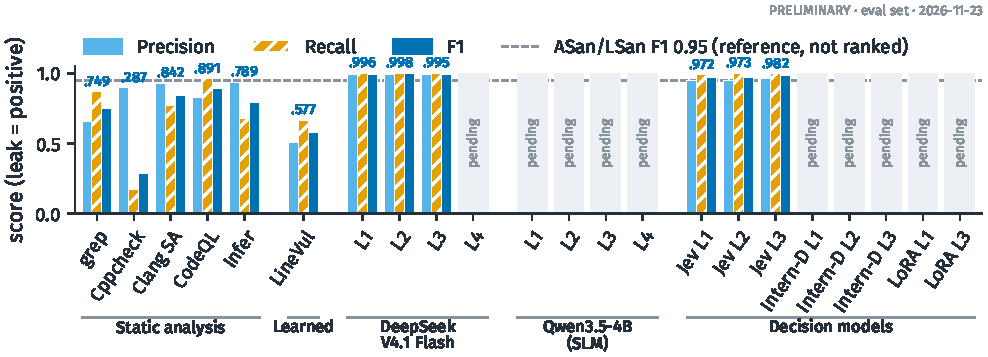
\includegraphics[width=\linewidth, height=0.62\textheight, keepaspectratio]{figures/prf1.pdf}
  \begin{itemize}\small
    \item grep drops to macro-F1 \res{grep}{macro} (was 0.940); LineVul is near chance; CodeQL is the best analyzer (F1 \res{codeql}{f1})
    \item DeepSeek L1/L2 reach F1 \res{deepseek_L1}{f1}\,/\,\res{deepseek_L2}{f1}, but Juliet is public: layer \ding{174} is the real test
  \end{itemize}
\end{frame}

% ------------------------------------------------------------------------------
\begin{frame}{Accuracy vs latency\prelim}
  \centering
  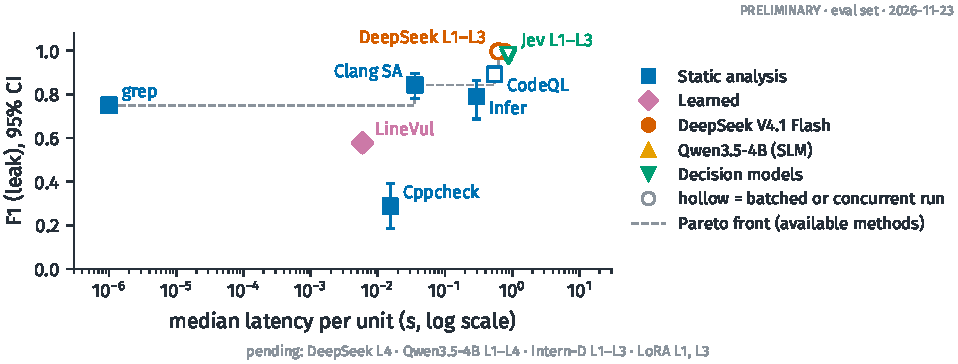
\includegraphics[width=\linewidth, height=0.65\textheight, keepaspectratio]{figures/pareto.pdf}
  \begin{itemize}\small
    \item Median per unit: Clang SA \res{clang_sa}{lat}\,s, CodeQL \res{codeql}{lat}\,s, DeepSeek L2 \res{deepseek_L2}{lat}\,s
    \item Hollow: batched or concurrent run, so latency is not per call at concurrency 1
  \end{itemize}
\end{frame}

% ------------------------------------------------------------------------------
\begin{frame}{Where do methods fail? F1 by flow category\prelim}
  \centering
  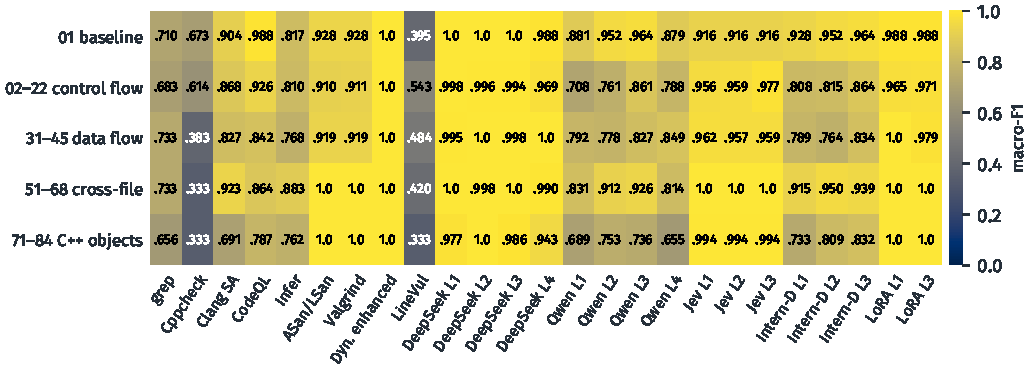
\includegraphics[width=\linewidth, height=0.6\textheight, keepaspectratio]{figures/heatmap.pdf}
  \begin{itemize}\small
    \item Cppcheck scores 0 on cross-file and C++ object code; Clang SA is weakest on C++ objects
    \item LLMs are near-uniform here, so per-category gaps must come from layers \ding{173}/\ding{174}
  \end{itemize}
\end{frame}
